\documentclass[class=NCU_thesis, crop=false]{standalone}
\begin{document}
	
\chapter{Results of monoHbb Analysis}\label{result}

\section{Main Uncertainties}
	The systematic uncertainties dominate the main uncertainty in this analysis. Among them, the b-tagging efficiency, the integrated luminosity, jet energy scale (JES) and jet energy resolution (JER) contribute the most to the experimental uncertainty. The SM predictions are the sources of the theoretical uncertainties. $t\bar{t}$ events, W/Z +jets events, associated production of SM Higgs boson decay into $b\bar{b}$ (Vh($b\bar{b}$), where V is the vector boson) and diboson events dominate the theoretical uncertainties.

	The uncertainty on the b-tagging efficiency originate from the flavor tagging efficiency in the $t\bar{t}$ events. A calibration, which highly makes use of beam testing in LHC, on the integrated luminosity is performed with a value a 2.0\%.

	The theoretical uncertainties originate from the SM modeling. Normalizations, acceptance difference and differential distributions of important kinematic variables derive the uncertainties.

	\section{Results}
		A fit to the invariant mass of Higgs candidate $m_h$ is used to search for the signal. For resolved region, $m_{\mathrm{jj}}$ represents the Higgs mass while $m_{\mathrm{J}}$ is used in the merged region.

		The fit is based on a LLH based approach. The systematic uncertainties are used in the likelihood function as nuisance parameters. The data in SR and two CRs are fit simultaneously for all four different (proxy) $E_T^{\mathrm{miss}}$ bins: $\left[150, 200\right)$ GeV, $\left[200, 350\right)$ GeV, $\left[350, 500\right)$ GeV, and $\left[500, \infty \right)$ GeV. $m_h$ is the fit variable in the SR. The fit variable used in the one-muon CR is the $\mu$ lepton charge. $t\bar{t}$ processes tend to produce the same amount of $\mu^+$ and $\mu^-$ leptons but the W+jets events produce more $\mu^+$ than $\mu^-$ leptons, which originates from proton-proton collision in LHC and from the conservation of electric charges. $\mu$-charge can thus be made use of as a differentiation of $t\bar{t}$ and W+jets events. In the two-lepton CR, the event yields serve as the fit variable because of limited data statistics.

		Figure \ref{fig:MET_SR} shows the $E_T^{\mathrm{miss}}$ distribution in SR. Figure \ref{fig:SR_mj} shows the distribution of $m_{\mathrm{jj}}$ or $m_{\mathrm{J}}$ in SR for resolved and merged region respectively. The data yields agree with the SM predictions. That is to say, no significant excess of the signal is found.

		An exclusion limit at 95\% confidence level (CL) is used for the interpretation of this analysis. The exclusion contour in $(m_{\mathrm{A}}, m_{\mathrm{Z'}})$ phase space is shown in figure \ref{fig:exclusion}. It also shows the result in the previous iteration. As it suggests, more region are excluded compared to the previous result. Figure \ref{fig:signal strength} shows the comparison of the upper limit of the signal strength between this result and the previous result, in which the fixed-radius (FR) track jets are used. In contrast to VR, FR track jets have a fixed cone size of $R = 0.2$. The plot also suggests more region in the phase space is excluded.

		\fig[0.6][fig:MET_SR][!hbt]{MET_SR.png}[The $E_T^{\mathrm{miss}}$ distribution for resolved and merged combined in SR. The dashed blue lines are the expectation yields before fits. The solid histograms are the simulations after fit. The dashed red lines are the expected signal from Z'-2HDM model.][short caption]

		\begin{figure}[!hbt]
			%\captionsetup[subfigure]{labelformat=empty} % hide figure's number.
			\centering
			\subcaptionbox
			{\label{fig:subfig_SR_mjj_150_200}}
			{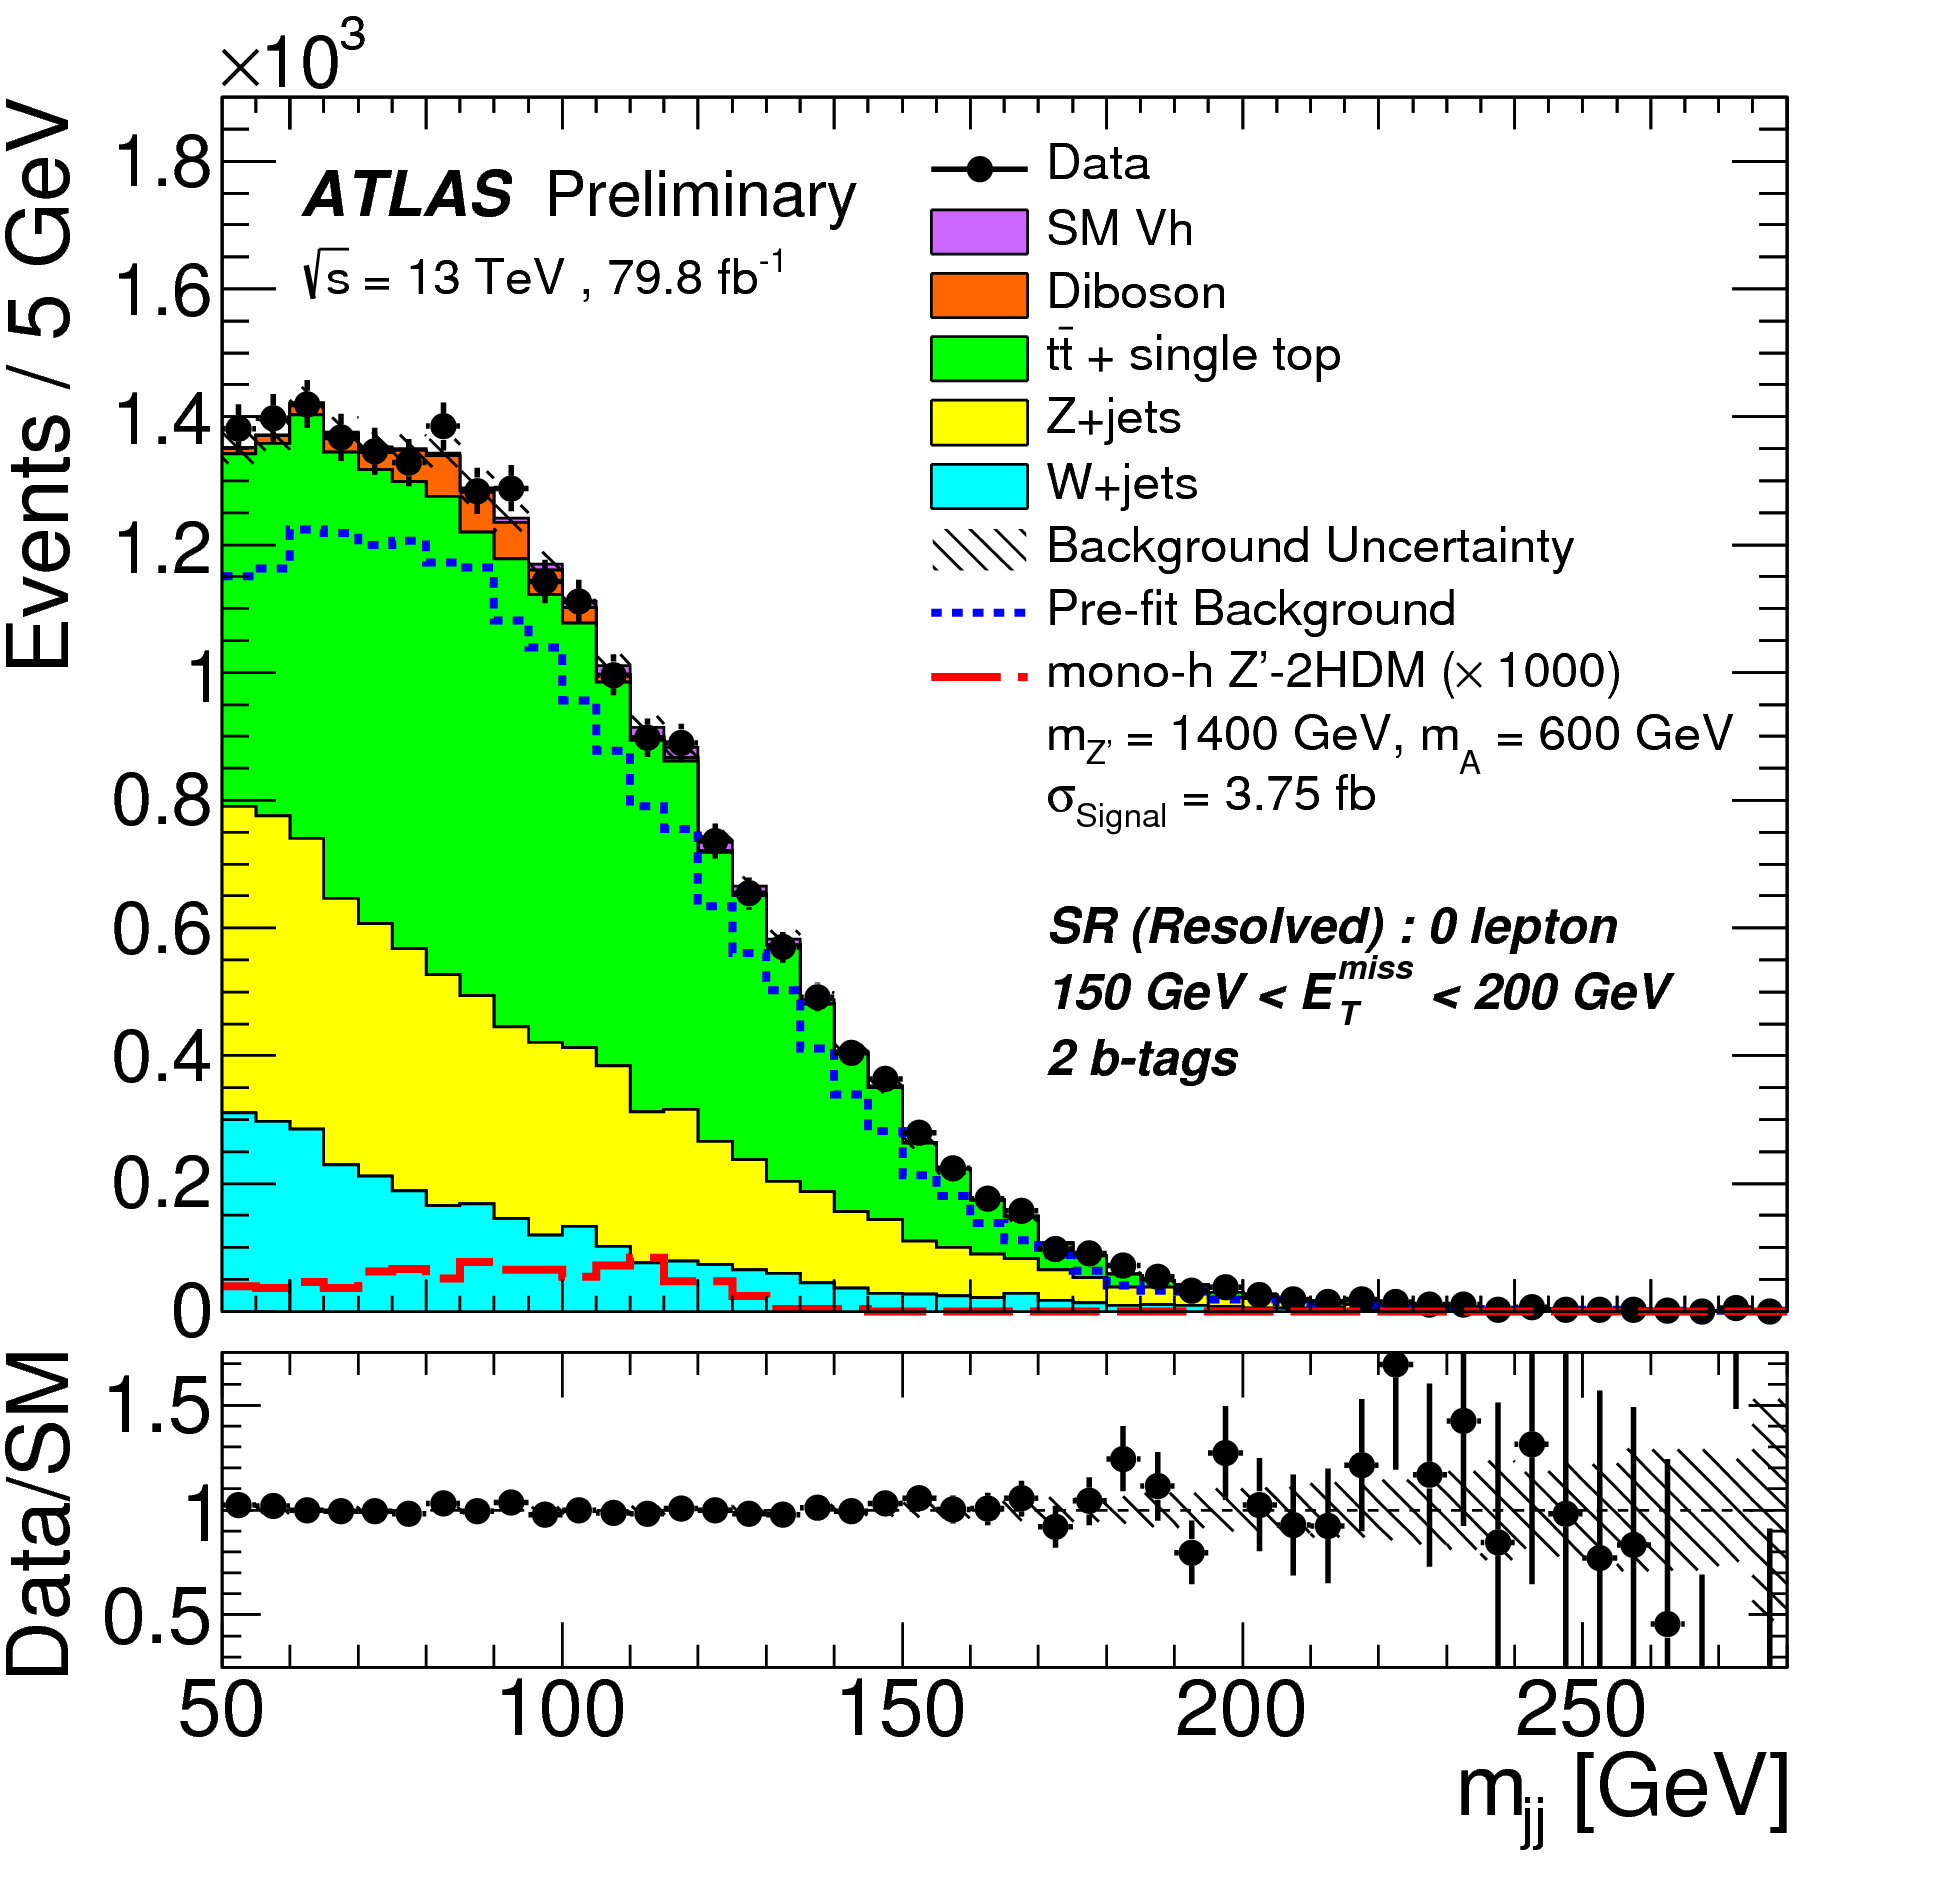
\includegraphics[width=0.4\linewidth]{SR_mjj_150_200.png}}
			~
			\subcaptionbox
			{\label{fig:subfig_SR_mjj_200_350}}
			{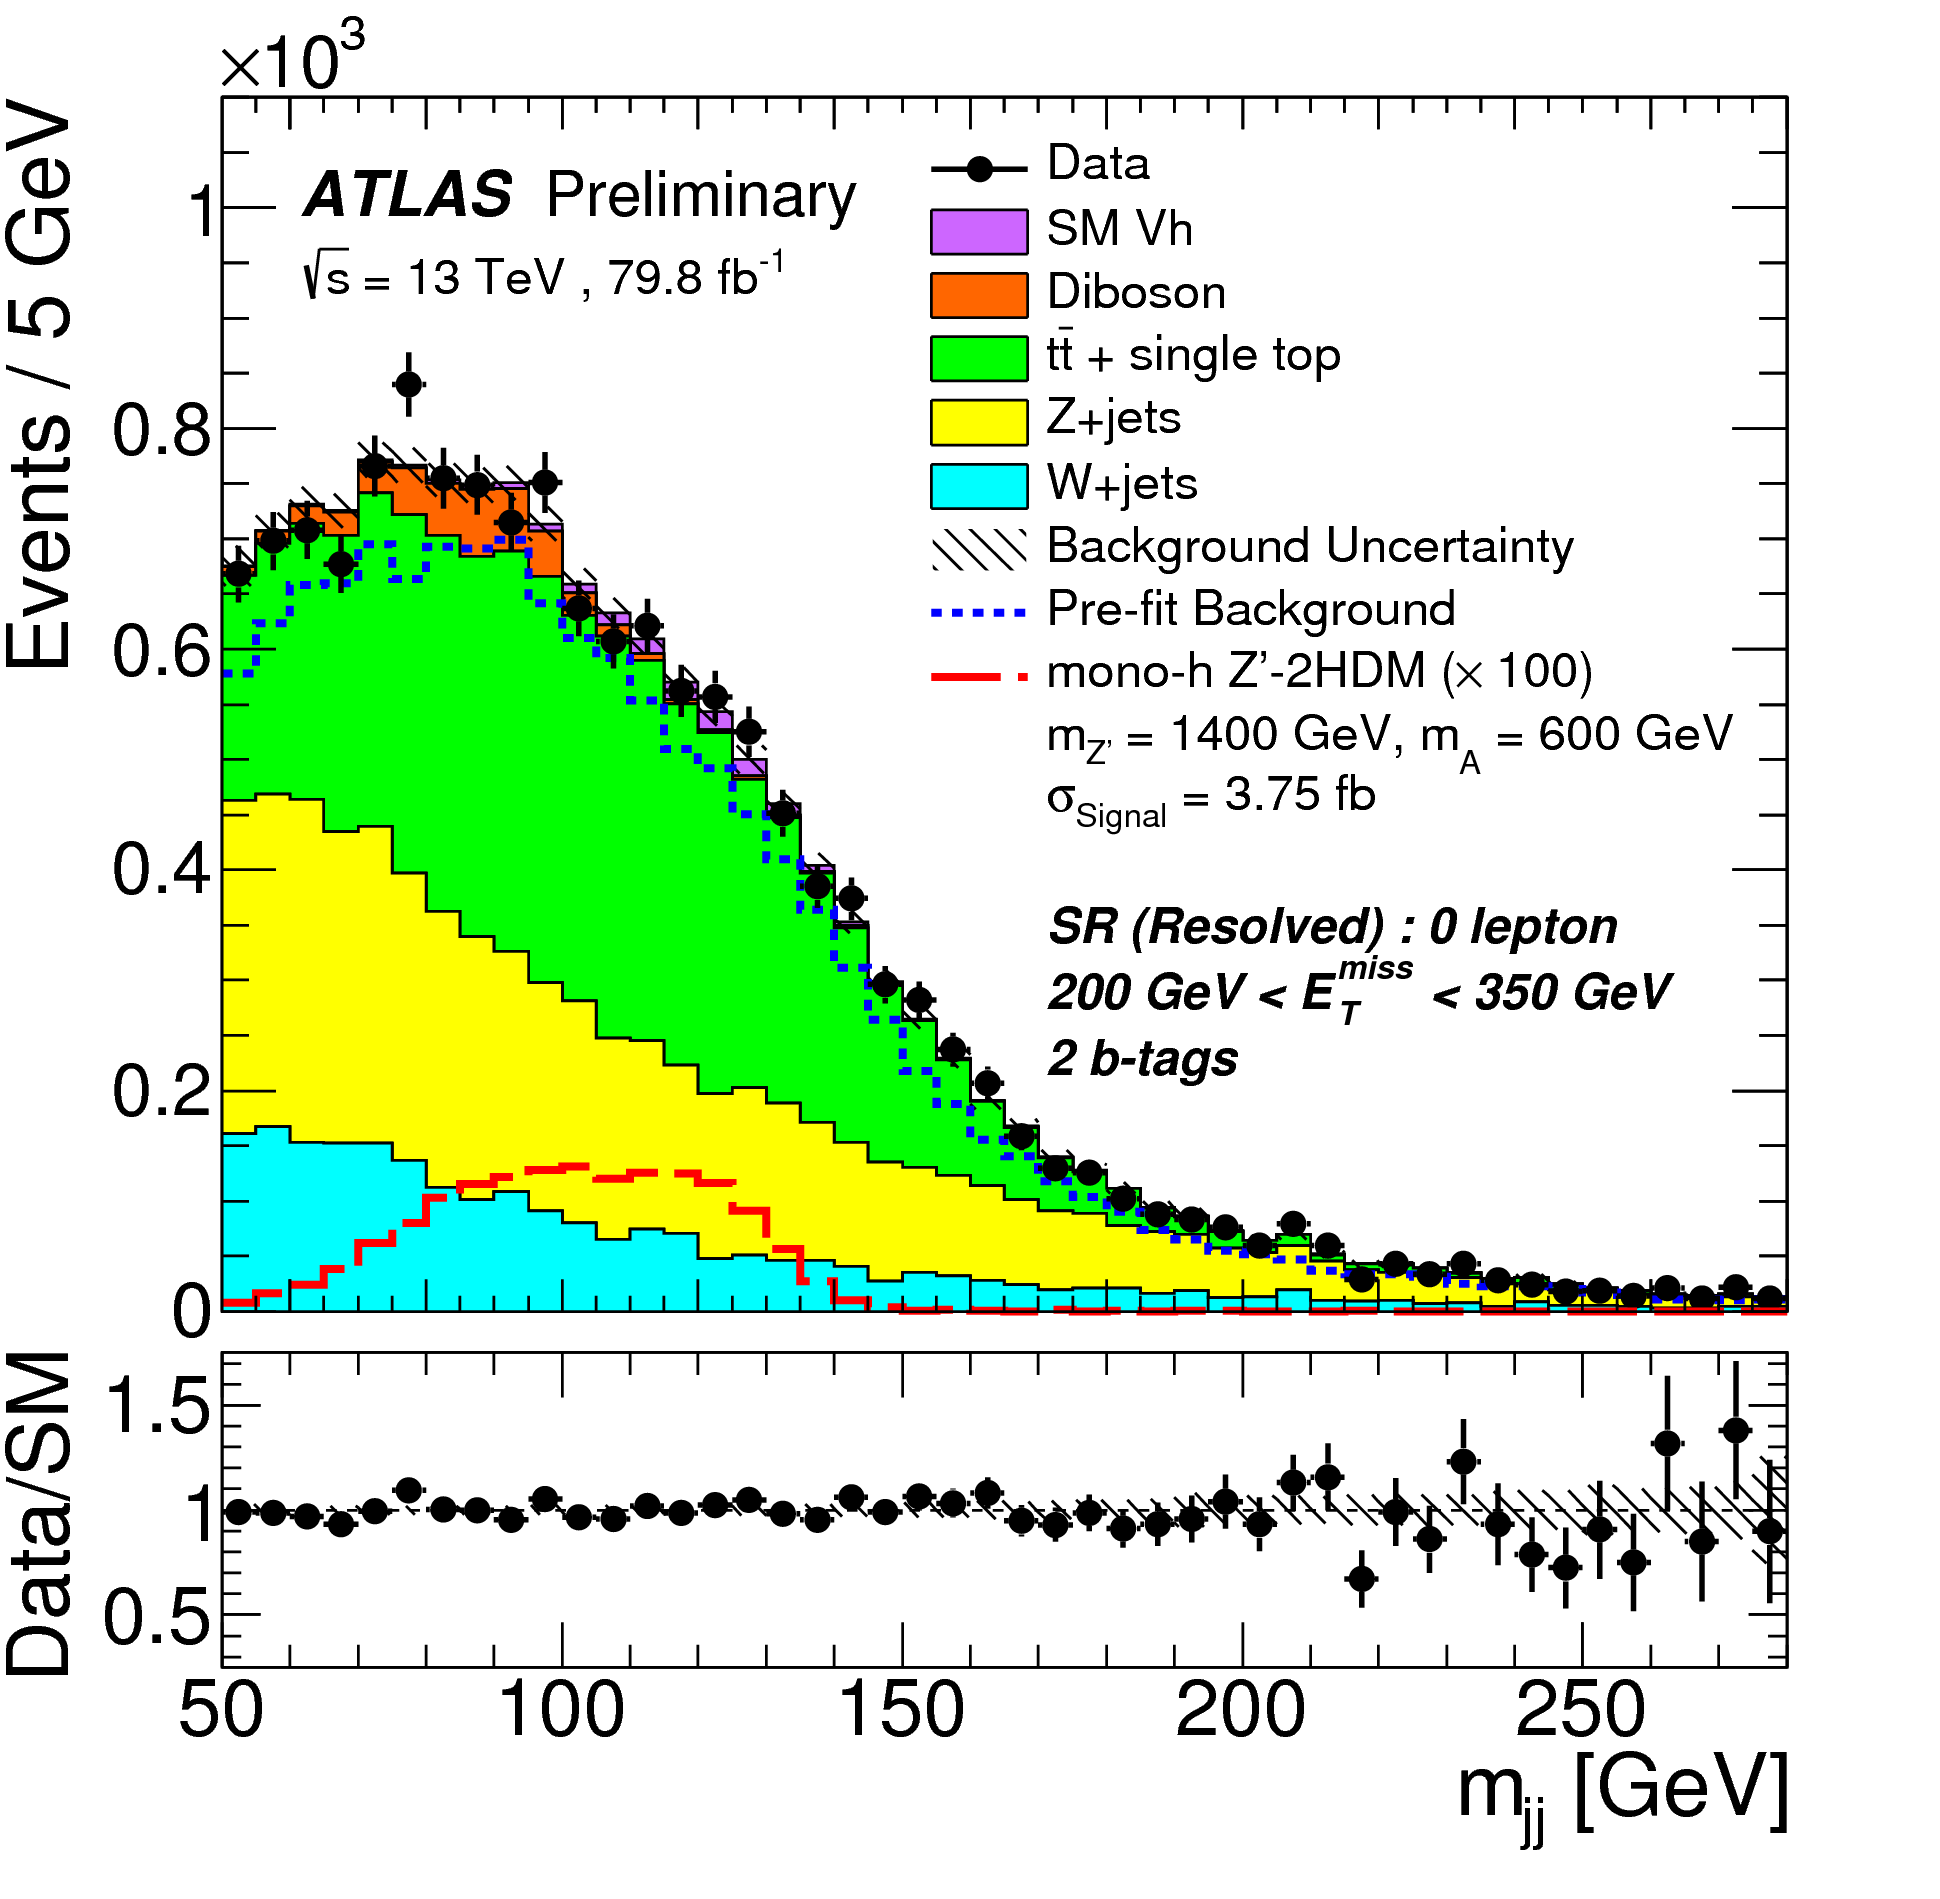
\includegraphics[width=0.4\linewidth]{SR_mjj_200_350.png}}
			\vspace{\baselineskip} % 分隔上下列
			\subcaptionbox
			{\label{fig:subfig_SR_mjj_350_500}}
			{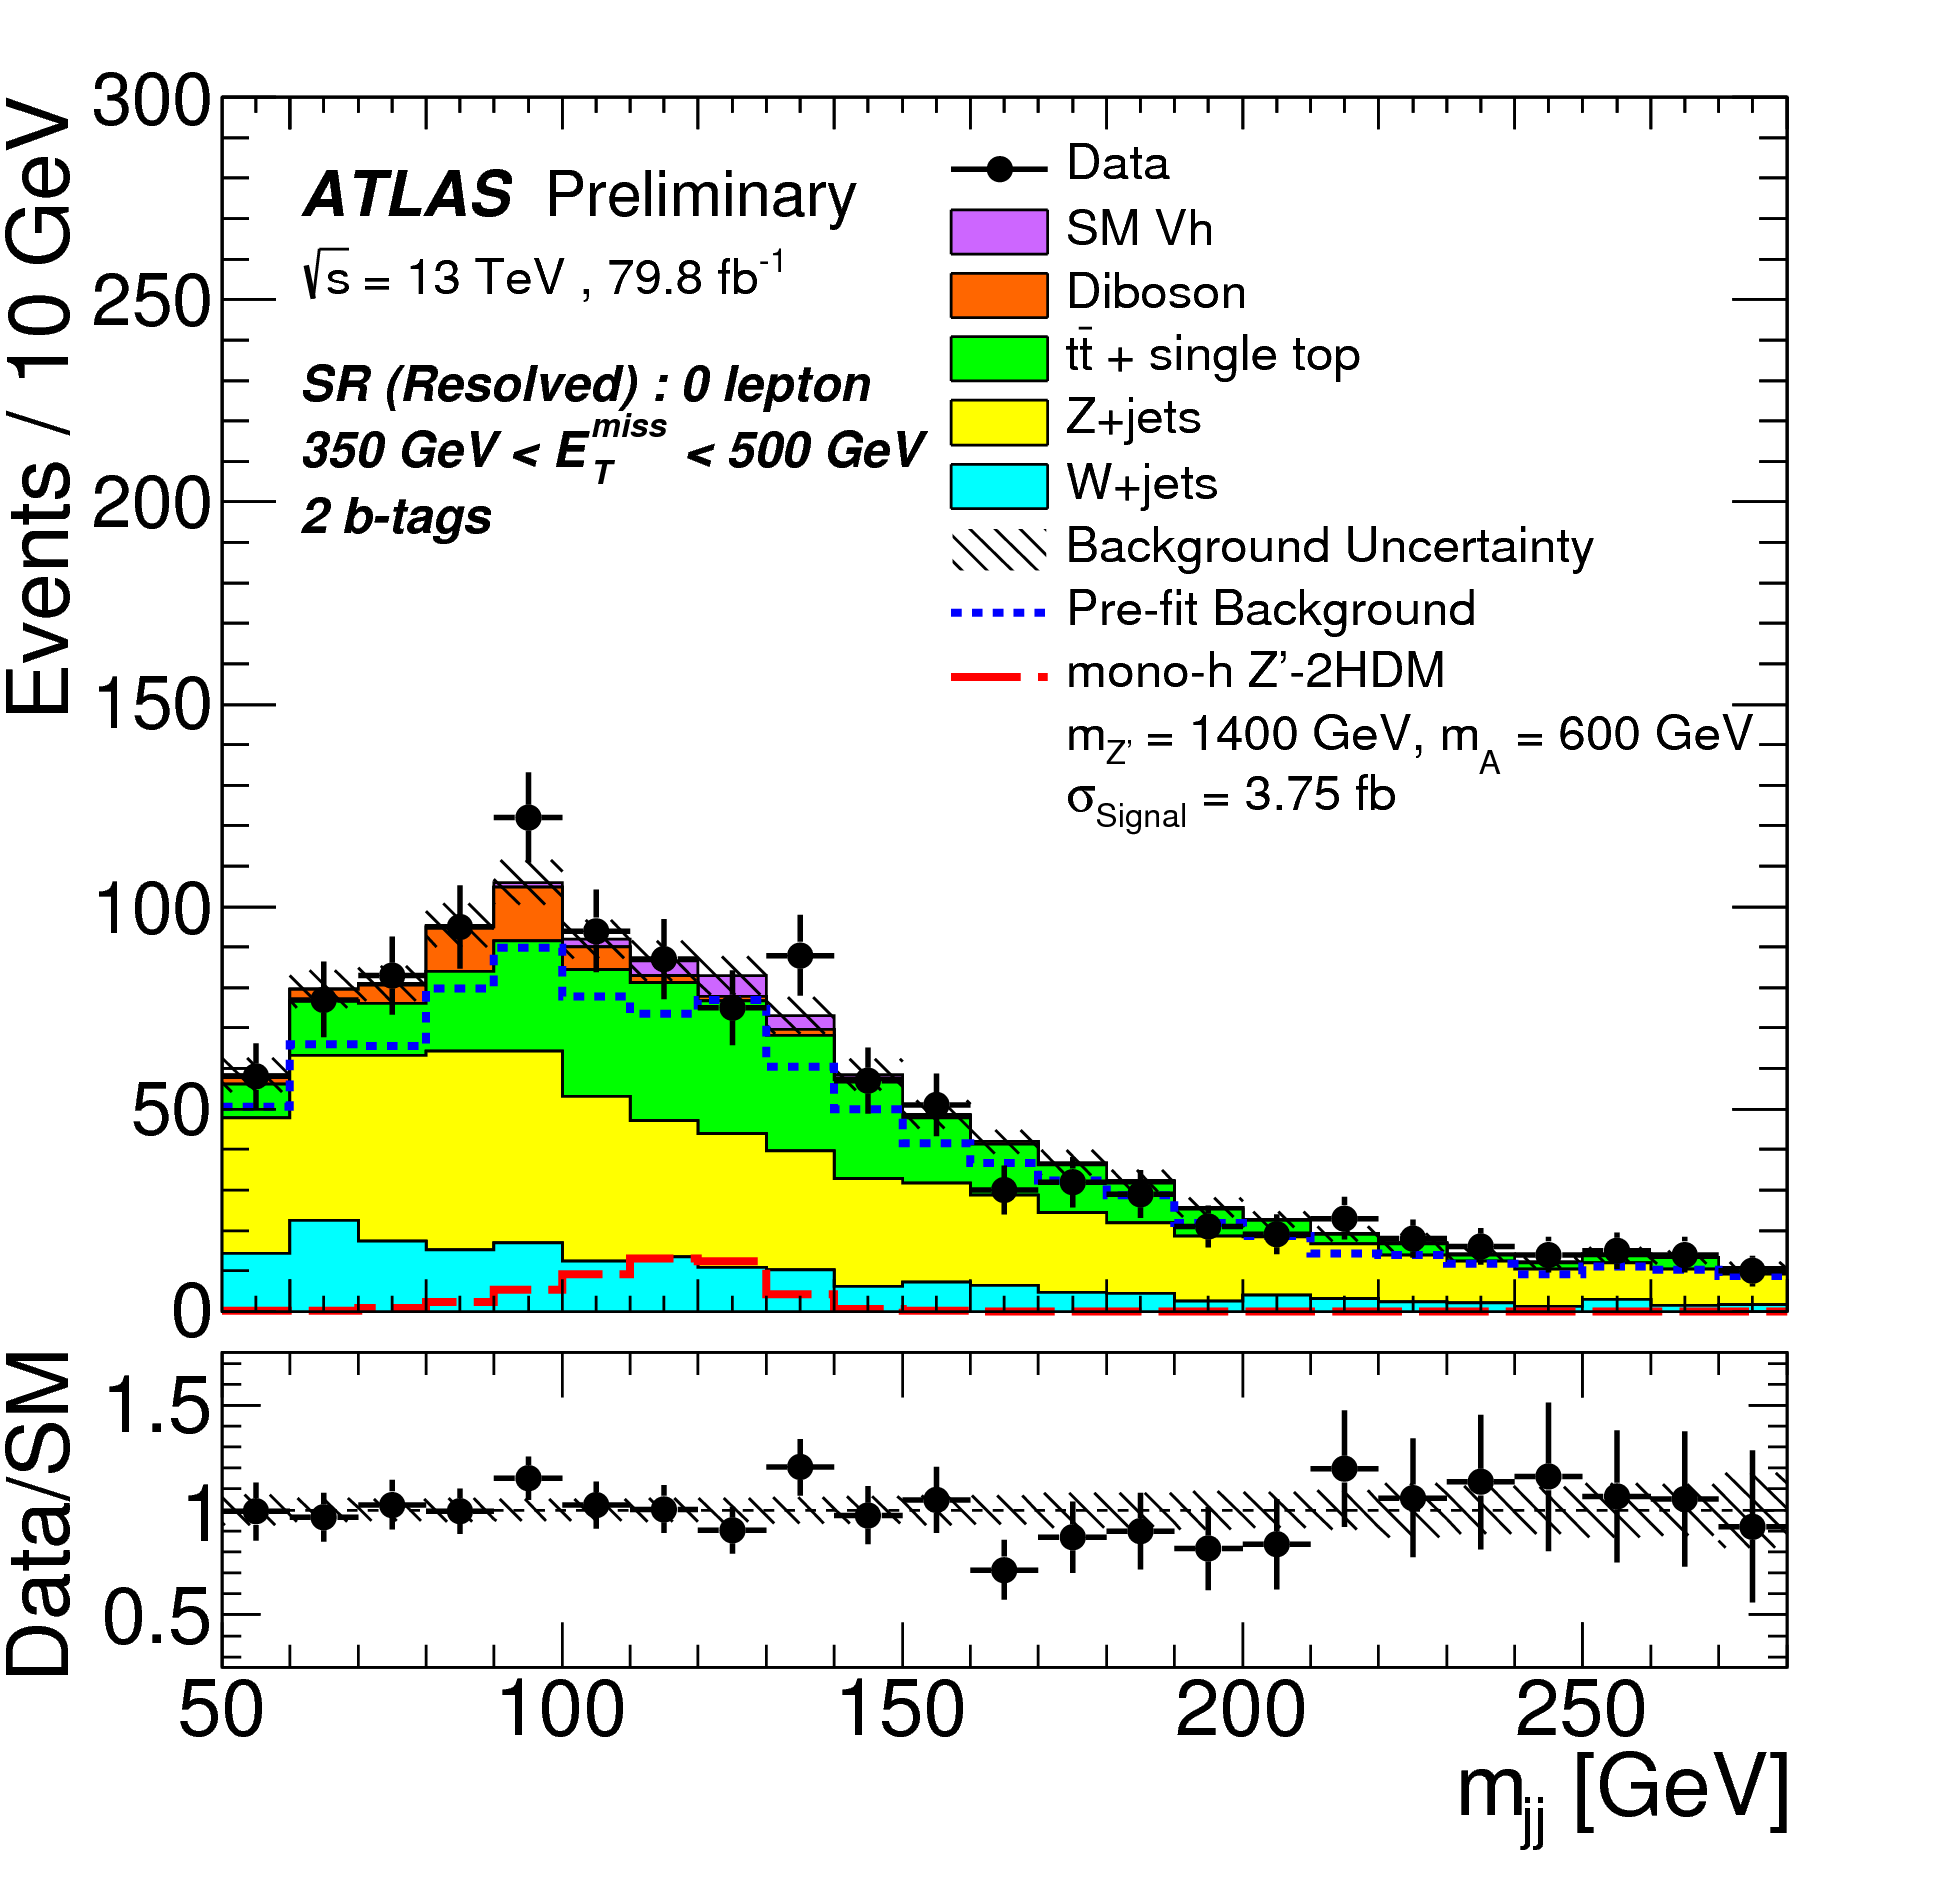
\includegraphics[width=0.4\linewidth]{SR_mjj_350_500.png}}
			\subcaptionbox
			{\label{fig:subfig_SR_mJ_500}}
			{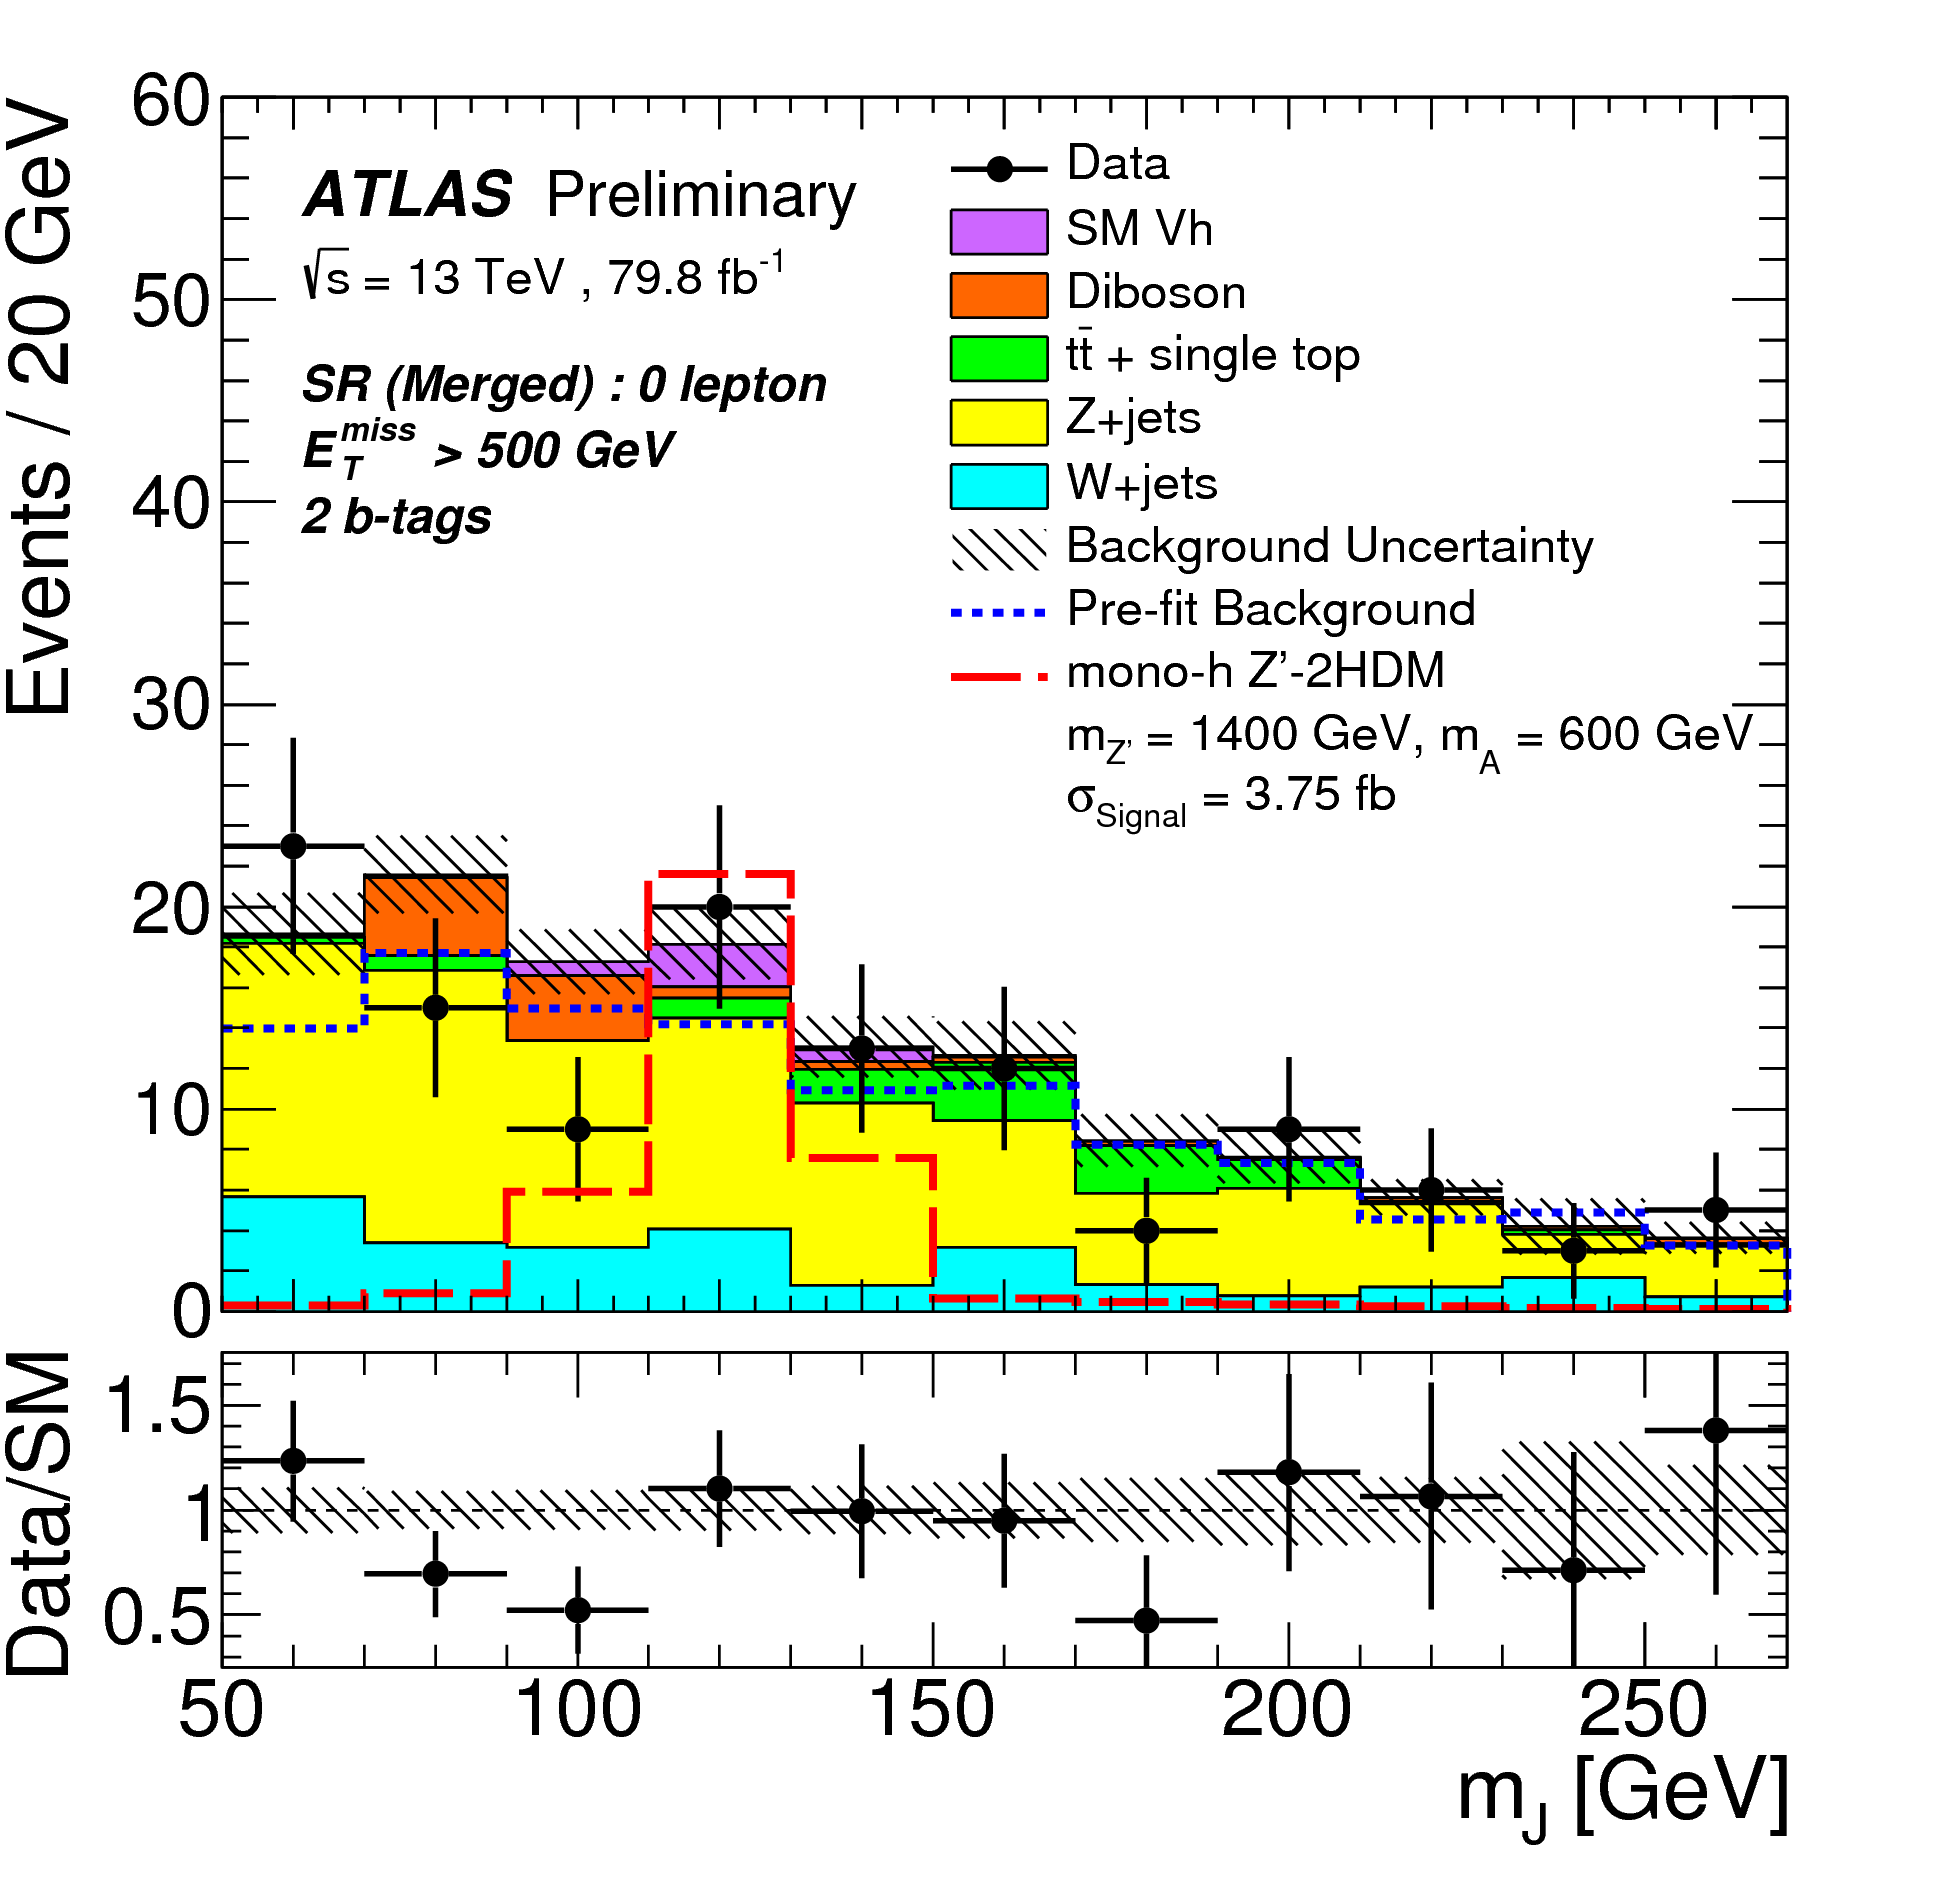
\includegraphics[width=0.4\linewidth]{SR_mJ_500.png}}
			\caption{Distirbution of the invariant mass of the Higgs boson candidate $m_{\mathrm{h}}$ with two b-tagged jets. The upper two plots are for $E_T^{\mathrm{miss}} \in \left[150, 200\right)$ GeV and $\left[200, 350\right)$ GeV bins. The lower two ones are for $E_T^{\mathrm{miss}} \in \left[350, 500\right)$ GeV and $\left[500, \infty \right)$ GeV. The dashed blue lines are the expectation yields before fits. The solid histograms are the simulations after fits. The dashed red lines are the expected signal from Z'-2HDM model. Its yields for the upper two plots are scaled up by a factor of 100 and 1000 from left to right respectively.}
			\label{fig:SR_mj}
		\end{figure}

		\fig[0.6][fig:exclusion][!hbt]{exclusion.png}[Exclusion contour in $(m_{\mathrm{A}}, m_{\mathrm{Z'}})$ phase space. Regions under the curve are excluded. The solid line shows consistency with SM-only hypothesis. The dashed blue line are the results from previous ATLAS results of $\sqrt{s} = 13$ TeV.][short caption]

		\fig[0.6][fig:signal strength][!hbt]{signal_strength.png}[The upper limit of the signal strength of this model with $m_{\mathrm{A}}$ fixed at 500 GeV. The dashed red line is the result of previous iteration, which made use of FR track jets. The dashed black line in the result of this iteration, where VR track jets are used. Signals, if exist, would appear in the region where the signal strength is greater than one. As a result, all regions whose upper limit is smaller than one is excluded. As the plot shows, making use of VR track jets extends the excluded region.][short caption]
		
\end{document}